\twocolumn[\colorsection{Preguntas para el análisis}]
\textit{En esta sección se requiere brindar respuestas argumentadas.}
\setcounter{figure}{0}
%
\begin{Exercise}
  Explique por qué no tendría sentido utilizar un termómetro de vidrio de tamaño normal, para medir la temperatura del agua caliente contenida en un dedal.
\end{Exercise}
%
\begin{Exercise}
  Si usted calienta el aire dentro de un recipiente rígido y sellado hasta que su temperatura en la escala Kelvin se duplique, la presión del aire en el recipiente también se duplica. ¿Esto es cierto si se duplica la temperatura Celsius del aire en el recipiente?
\end{Exercise}
%
\begin{Exercise}
  \textit{a}) Suponga que en el problema \ref{p:calorimetria01} no es posible despreciar la transferencia de calor del líquido al recipiente en ese experimento. ¿El resultado obtenido en dicho experimento, es mayor o menor que el calor específico promedio real del líquido? \textit{b}) Ahora suponga que se puede despreciar el intercambio de calor con el recipiente, pero no es posible despreciar el intercambio de calor con el entorno. ¿El resultado obtenido en dicho experimento, es mayor o menor que el calor específico promedio real del líquido?
\end{Exercise}
%
\begin{Exercise}
  Si en el problema \ref{p:transmision00} se tuviera en cuenta la convección del aire a ambos lados de la pared, ¿la corriente de calor sería mayor, menor o la misma que la calculada en dicho problema?
\end{Exercise}
%
\begin{Exercise}
  Se desea cubrir las paredes metálicas de un horno con un material aislante. ¿Cuáles de los siguientes valores cambian y cuáles se mantienen igual si en lugar de aplicar el revestimiento en el interior del horno se lo aplica sobre el exterior de las paredes?: \textit{i}) la potencia transmitida a través de las paredes; \textit{ii}) la temperatura de la superficie interior; \textit{iii}) la temperatura de la superficie exterior. ¿Sus respuestas son las mismas si se incluye o no convección en los cálculos?
\end{Exercise}
%
\begin{Exercise}\label{p:preguntastermo01}
  \ifthenelse{\equal{\seleccionados}{true}}
  {\addToList{xyz-preguntas}{\ExerciseHeaderNB}}{}
  En la figura \ref{f:preguntastermo01} se muestra la evolución de la temperatura en función del calor intercambiado con el entorno para una muestra de un líquido desconocido. Si $\text{C}_{\text{l}}$ es el calor específico de este líquido y $\text{C}_{\text{s}}$ es el calor específico de la misma sustancia en estado sólido, ¿cuál de las siguientes opciones es la única correcta?\\
\renewcommand{\arraystretch}{1.5}
  \begin{tabular}{p{2.5cm} p{2.5cm} p{2.5cm}}
     \textit{a}) $\text{C}_{\text{s}}=\text{C}_{\text{l}}$ & \textit{b}) $\text{C}_{\text{s}}=3\text{C}_{\text{l}}$ & \textit{c}) $\text{C}_{\text{s}}=\text{C}_{\text{l}}/3$ \\
     \textit{d}) $\text{C}_{\text{s}}=9\text{C}_{\text{l}}$ & e) $\text{C}_{\text{s}}=\text{C}_{\text{l}}/9$ \\
  \end{tabular} \\
\end{Exercise}
%
\begin{center}
    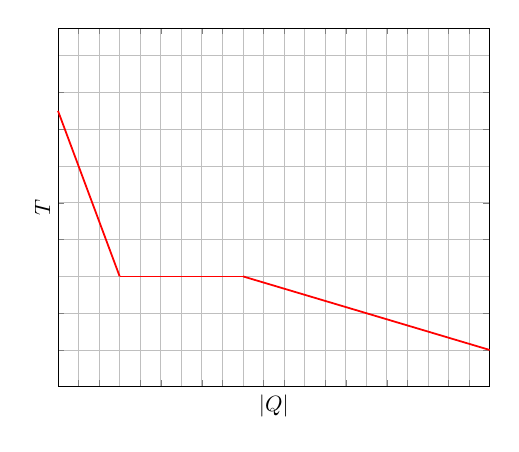
\begin{tikzpicture}[scale=0.8]
        \begin{axis}[
            ticks= none,
            every major x tick/.append style={thick,blue},
            clip=false,
            grid=both,
            minor x tick num=2,        
            minor y tick num=2,
            xmin=0, xmax=7,   
            ymin=0, ymax=6.5,
            %xtick  align=center,
            xlabel={$|Q|$},
            ylabel={$T$}
        ];
        \addplot [color=red, thick] [id=p36a,samples= 180, domain=0:1]  {5-3*x};
        \addplot [color=red, thick] [id=p36b,samples= 180, domain=1:3]  {2};
        \addplot [color=red, thick] [id=p36c,samples= 180, domain=3:7]  {2-1/3*(x-3)};
        \end{axis}
    \end{tikzpicture}
    \captionof{figure}{Pregunta \ref{p:preguntastermo01}\label{f:preguntastermo01}}
\end{center}
%
\begin{Exercise}
  ¿Es correcto afirmar que si se disminuye el área de un cuerpo, el calor intercambiado disminuye en la misma proporción independientemente del mecanismo considerado?
\end{Exercise}
%
\begin{Exercise}
  \textit{a}) Un bloque de metal frío se siente más frío que uno de madera a la misma temperatura. ¿Por qué? \textit{b}) Un bloque de metal caliente se siente más caliente que uno de madera a la misma temperatura. ¿Por qué? \textit{c}) ¿Hay alguna temperatura a la que ambos bloques se sientan igualmente calientes o fríos? ¿Cuál es esta?
\end{Exercise}
%
\begin{Exercise}
  En algunas situaciones suele considerarse que uno de los mecanismos de transmisión del calor es ``más importante'' que los otros. \textit{a}) Mencione un caso en que la conducción es el mecanismo primordial y de algunas razones para que esta aproximación pueda considerarse correcta. \textit{b}) Ídem \textit{a}) para convección. \textit{c}) Ídem \textit{a}) para radiación.
\end{Exercise}
%
\begin{Exercise}\label{p:preguntastermo02}
  \ifthenelse{\equal{\seleccionados}{true}}
  {\addToList{xyz-preguntas}{\ExerciseHeaderNB}}{}
  El gráfico de la figura \ref{f:preguntastermo02} representa la temperatura en función a la distancia a la fuente caliente dentro de una pared formada por dos materiales, el material $A$ con un espesor $l$ y el material $B$ con espesor $2l$. Para el gráfico en cuestión analice las siguientes afirmaciones y diga si son verdaderas o falsas y por qué: \textit{a}) La conductividad térmica de $A$ es mayor que la de $B$. \textit{b}) La temperatura de unión en la superficie de contacto antre $A$ y $B$ es menor que el promedio de las temperaturas en los lados de la pared. \textit{c}) El flujo calórico es mayor en el material de mayor conductividad.
\end{Exercise}
%
\begin{center}
  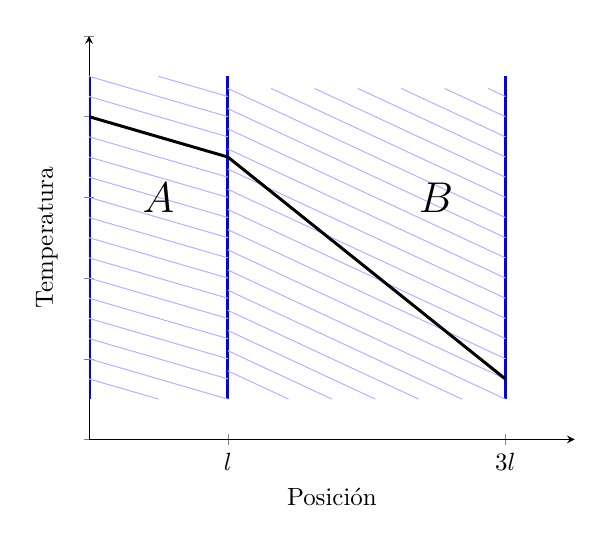
\begin{tikzpicture}[scale=0.9]
    \begin{axis}[
      %ticks=none,
      axis x line=bottom,
      axis y line=left,
      xmin=0, xmax=3.5,
      ymin=0, ymax=5,
      xlabel={Posición},
      ylabel={Temperatura},
      xtick={1,3},
      xticklabels={$l$,$3l$},
      ytick={},
      yticklabels={}
      ];
    \draw [color=blue, very thick](0,0.5)--(0,4.5);
    \draw [color=blue, very thick](1,0.5)--(1,4.5);
    \draw [color=blue, very thick](3,0.5)--(3,4.5);

    % No puedo usar foreach adentro de axis, y si lo uso afuera no
    % respeta la escala.
    \draw [color=blue!30](0,0.75)--(0.5,0.5);
    \draw [color=blue!30](0,1)--(1,0.5);
    \draw [color=blue!30](0,1.25)--(1,0.75);
    \draw [color=blue!30](0,1.5)--(1,1);
    \draw [color=blue!30](0,1.75)--(1,1.25);
    \draw [color=blue!30](0,2)--(1,1.5);
    \draw [color=blue!30](0,2.25)--(1,1.75);
    \draw [color=blue!30](0,2.5)--(1,2);
    \draw [color=blue!30](0,2.75)--(1,2.25);
    \draw [color=blue!30](0,3)--(1,2.5);
    \draw [color=blue!30](0,3.25)--(1,2.75);
    \draw [color=blue!30](0,3.5)--(1,3);
    \draw [color=blue!30](0,3.75)--(1,3.25);
    \draw [color=blue!30](0,4)--(1,3.5);
    \draw [color=blue!30](0,4.25)--(1,3.75);
    \draw [color=blue!30](0,4.5)--(1,4);
    \draw [color=blue!30](0.5,4.5)--(1,4.25);

    \draw [color=blue!30](2.875,4.35)--(3,4.25);
    \draw [color=blue!30](2.5625,4.35)--(3,4);
    \draw [color=blue!30](2.25,4.35)--(3,3.75);
    \draw [color=blue!30](1.9375,4.35)--(3,3.5);
    \draw [color=blue!30](1.625,4.35)--(3,3.25);
    \draw [color=blue!30](1.3125,4.35)--(3,3);
    \draw [color=blue!30](1,4.35)--(3,2.75);
    \draw [color=blue!30](1,4.10)--(3,2.5);
    \draw [color=blue!30](1,3.85)--(3,2.25);
    \draw [color=blue!30](1,3.60)--(3,2.0);
    \draw [color=blue!30](1,3.35)--(3,1.75);
    \draw [color=blue!30](1,3.10)--(3,1.5);
    \draw [color=blue!30](1,2.85)--(3,1.25);
    \draw [color=blue!30](1,2.6)--(3,1.);
    \draw [color=blue!30](1,2.35)--(3,0.75);
    \draw [color=blue!30](1,2.10)--(3,0.5);
    \draw [color=blue!30](1,1.85)--(2.6875,0.5);
    \draw [color=blue!30](1,1.6)--(2.375,0.5);
    \draw [color=blue!30](1,1.35)--(2.0625,0.5);
    \draw [color=blue!30](1,1.1)--(1.75,0.5);
    \draw [color=blue!30](1,0.85)--(1.4375,0.5);

    \draw [color=black, very thick](0,4)--(1,3.5);
    \draw [color=black, very thick](1,3.5)--(3,0.75);

    \draw (0.5,3) node [font=\fontsize{17}{0}] {$A$};
    \draw (2.5,3) node [font=\fontsize{17}{0}] {$B$};
    \end{axis}
    % \foreach \y in {1,...,5}
    %     \draw [color=blue!30](0,\y)--(1.8,\y-0.5);
  \end{tikzpicture}
  \captionof{figure}{Problema \ref{p:preguntastermo02}\label{f:preguntastermo02}}
\end{center}
%
\begin{Exercise}\label{p:preguntastermo03}
  En la figura \ref{f:preguntastermo03} se muestran dos evoluciones de un mismo gas ideal. ¿Cómo se comparan el calor $Q_{a\rightarrow b \rightarrow c}$ a lo largo de la línea sólida con el calor $Q_{a\rightarrow c}$ a lo largo de la línea punteada?
\end{Exercise}
%
\begin{center}
  \begin{tikzpicture}[scale=0.9]
    \begin{axis}[
      ticks=none,
      axis x line=bottom,
      axis y line=left,
      clip=false,
      xmin=0, xmax=1.1,
      ymin=0, ymax=4.5,
      xtick  align=center,
      xlabel={$V$},
      ylabel={$p$}
      ];
      \draw [color=blue, very thick][-latex](0.2,1)--(0.4,2.5);
      \draw [color=blue, very thick](0.4,2.5)--(0.6,4);
      \draw [color=blue, very thick][-latex](0.6,4)--(0.8,2.5);
      \draw [color=blue, very thick](0.8,2.5)--(1,1);
      \draw [color=blue, dashed, very thick][-latex](0.2,1)--(0.6,1);
      \draw [color=blue, dashed, very thick](0.6,1)--(1,1);
      \draw (0.2,1) node [below left] {$a$};
      \draw (0.6,4) node [above left] {$b$};
      \draw (1,1) node [below right] {$c$};
      \fill [black](0.2,1) circle(2pt);
      \fill [black](0.6,4) circle(2pt);
      \fill [black](1,1) circle(2pt);
    \end{axis}
  \end{tikzpicture}
  \captionof{figure}{Problema \ref{p:preguntastermo03}\label{f:preguntastermo03}}
\end{center}
%
\begin{Exercise}
  \ifthenelse{\equal{\seleccionados}{true}}
  {\addToList{xyz-preguntas}{\ExerciseHeaderNB}}{}
  En un calorímetro ideal se mezclan una masa de agua a $\SI{70}{\celsius}$ y otra masa de agua a $\SI{20}{\celsius}$, y se espera hasta que el sistema (la mezcla) alcance el equilibrio térmico. Siendo que el sistema está aislado del entorno, ¿varía su entropía?
\end{Exercise}
%
\begin{Exercise}
  En los siguientes procesos, ¿el trabajo efectuado por el sistema (definido como un gas que se expande o se contrae) sobre el ambiente es positivo o negativo? \textit{a}) La expansión de una mezcla aire-gasolina quemada en el cilindro de un motor de automóvil; \textit{b}) abrir una botella de champaña; \textit{c}) llenar un tanque de buceo con aire comprimido; \textit{d}) la abolladura parcial de una botella de agua vacía y cerrada, al conducir descendiendo desde las montañas hacia el nivel del mar.
\end{Exercise}
%
\begin{Exercise}
  ¿En qué situación debe usted efectuar más trabajo: al inflar un globo al nivel del mar o al inflar el mismo globo con el mismo volumen en la cima del Aconcagua?
\end{Exercise}
%
\begin{Exercise}
  \ifthenelse{\equal{\seleccionados}{true}}
  {\addToList{xyz-preguntas}{\ExerciseHeaderNB}}{}
  Cuando se derrite hielo a $\SI{0}{\celsius}$ su volumen disminuye. ¿El cambio de energía interna es mayor, menor o igual que el calor agregado?
\end{Exercise}
%
\begin{Exercise}
  Un gas ideal se expande mientras que la presión se mantiene constante. Durante este proceso, ¿hay flujo de calor hacia el gas o hacia afuera de este?
\end{Exercise}
%
\begin{Exercise}
  En un proceso a volumen constante, $dU = nC_VdT$. En cambio, en un proceso a presión constante, no se cumple que $dU = nC_pdT$. ¿Por qué no?
\end{Exercise}
%
\begin{Exercise}
  Convertir energía mecánica totalmente en calor, ¿viola la segunda ley de la termodinámica? ¿Y convertir calor totalmente en trabajo?
\end{Exercise}
%
\begin{Exercise}\label{p:preguntastermo04}
  Un sistema termodinámico experimenta un proceso cíclico como se muestra en la figura \ref{f:preguntastermo04}. El ciclo consiste en dos lazos cerrados: el lazo \textit{I} y el \textit{II}. \textit{a}) Durante un ciclo completo, ¿el sistema efectúa trabajo neto positivo o negativo? \textit{b}) Durante un ciclo completo, ¿entra calor al sistema o sale de él? \textit{c}) En cada lazo, \textit{I} y \textit{II}, ¿entra calor en el sistema o sale de él?
\end{Exercise}
%
% It needs \usetikzlibrary{decorations.markings}
% and the tikzet defined in the preamble.
\begin{center}
  \begin{tikzpicture}[scale=0.9]
    \draw [cyan] plot [smooth cycle, tension=1] coordinates { (0,0.5) (2,2.5) (3,-2) (4.5,-2.4)} [arrow inside={end=stealth,opt={red,scale=2}}{0,0.35,0.5,0.75}];
    \draw [-latex] (-1,-3.5) -- (-1,3.5) node [left] {$p$};
    \draw [-latex] (-1,-3.5) -- (5.5,-3.5) node [below] {$V$};
    \draw (1.35,1) node [] {$I$};
    \draw (4,-2.5) node [] {$II$};
  \end{tikzpicture}
  \captionof{figure}{Problema \ref{p:preguntastermo04}\label{f:preguntastermo04}}
\end{center}
%
\begin{Exercise}
  \ifthenelse{\equal{\seleccionados}{true}}
  {\addToList{xyz-preguntas}{\ExerciseHeaderNB}}{}
  Compare el diagrama $p$-$V$ para el ciclo Otto con el diagrama para la máquina térmica de Carnot. Explique algunas diferencias importantes entre los dos ciclos.
\end{Exercise}
%
\begin{Exercise}
  ¿Puede un sistema experimentar variaciones de entropía negativas?
\end{Exercise}
%
\begin{Exercise}
  ¿Un refrigerador lleno de alimentos con una temperatura ambiente de $\SI{20}{\celsius}$ consume más potencia si la temperatura es de $\SI{15}{\celsius}$? ¿O el consumo es el mismo?
\end{Exercise}
%
\begin{Exercise}
  Explique si en cada uno de los siguientes procesos hay aumentos de entropía o no: la mezcla de agua caliente y fría; expansión libre de un gas; flujo irreversible de calor; producción de calor por fricción mecánica.
\end{Exercise}
%
\begin{Exercise}
  La expansión libre de un gas ideal es un proceso adiabático, por lo que no hay transferencia de calor. Tampoco se realiza trabajo, de manera que la energía interna no cambia. Por lo tanto, $Q/T = 0$; sin embargo, la entropía es mayor después de la expansión. ¿Por qué la ecuación $\Delta S = \int dQ/T$ no se aplica a esta situación?
\end{Exercise}
%
